  \begin{section}{Die Konfigurationen}
   Eine Klasse von Graphen ist für den Beweis des Vier-Farben-Satzes wesentlich: Die Konfigurationen. Sie treten vor allem als Untergraphen der normalen Graphen auf. Zuerst wollen wir festhalten, was eine Konfiguration eigentlich ist.
   
   \begin{definitionl}{Konfiguration}{konfig}
    Ein Graph $C$ heißt \textit{Konfiguration}, wenn
    \begin{itemize}
     \item er regulär ist,
     \item die Außenknoten einen Ring der \textit{Ringgröße} $k \geq 4$ bilden,
     \item innere Knoten existieren,
     \item die beschränkten Gebiete von Dreiecken begrenzt werden,
     \item jedes Dreieck Grenze eines Gebiets ist.
    \end{itemize}
   \end{definitionl}
   
  Um eine bessere Vorstellung für diese Graphen zu bekommen, betrachten wir zunächst einige Beispiele. Ein nicht-triviales Beispiel für eine Konfiguration ist der \textit{Birkhoff}-Diamant mit insgesamt 10 Knoten.
   
  \[  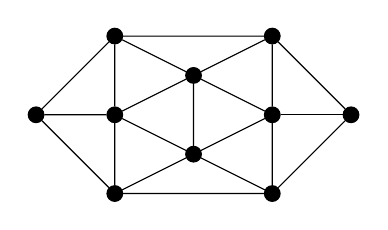
\begin{tikzpicture}[every node/.style={draw,inner sep=2pt,fill=black}]
      \path[shape=circle]
	(0,1) node(a1){} 
	(1,0) node(b1){} (1,1) node(b2){} (1,2) node(b3){}
	(2,0.5) node(c1){} (2,1.5) node(c2){}
	(3,0) node(d1){} (3,1) node(d2){} (3,2) node(d3){}
	(4,1) node(e1){};
	\filldraw (a1) -- (b1) -- (d1) -- (e1) -- (d3) -- (b3) -- (a1) -- (b2);
	\filldraw (b1) -- (b2) -- (b3) -- (c2) -- (d3) -- (d2) -- (d1) -- (c1) -- (b1);
	\filldraw (c1) -- (b2) -- (c2) -- (c1);
	\filldraw (c1) -- (d2) -- (c2);
	\filldraw (d2) -- (e1);
    \end{tikzpicture}   \]
   
  Andere Beispiele für Konfigurationen sind \textit{Sterne}. Sie besitzen genau einen inneren Punkt (``\textit{Zentrum}'') und einen Ring von äußeren Punkten, die alle mit dem Zentrum durch eine Kante verbunden sind. Ein Stern heißt $k$-Stern, wenn er genau $k$ äußere Knoten besitzt.
  
  \begin{definition}{Äquivalente Konfigurationen}
   Zwei Konfigurationen $C'=(V',E')$ und $C''=(V'',E'')$ heißen \textit{äquivalent}, wenn es eine Bijektion $\varphi : V' \rightarrow V''$ gibt, die in beide Richtungen die Adjazenzstruktur erhält.
  \end{definition}
  
  Nun können wir davon sprechen, dass ein Graph eine Konfiguration enthält, indem wir folgende Definition bemühen:
  
  \begin{definition}{enthaltene Konfiguration}
   Man sagt, ein Graph $G$ \textit{enthält} eine Konfiguration $C$, wenn es einen geschlossenen Pfad $K$ gibt, sodass der von den Knoten von $K$ und den im Innengebiet liegenden Knoten von $K$ Untergraph $C_K$ von $G$ eine zu $C$ äquivalente Konfiguration ist.
  \end{definition}


  \end{section}
\newpage